\section{Evaluation}
\label{Sec:Evaluation}

	\subsection{Goals and Research Questions}
	\label{Sec:Goals}
	In order to evaluate how effective is our tool in assisting the developers, we empirically evaluated our tool as well as conducted an a user study. We wish to answer the following research questions in our study.
	\begin{description}
		\item[RQ1:] What is the convergence rate for number of unique CSS selectors verses number of DOM states?
		\item[RQ2:] How accurate are the code-completion suggestions provided by the tool?
		\item[RQ3:] How is the list of code-completion suggestions affected by each phase of our analysis?
		\item[RQ4:] Does \dompletion make programming tasks faster without compromising correctness of the program?
		\item[RQ5:] Does \dompletion make debugging tasks easier?
%		\item[RQ5:] What is the overhead
		
	\end{description}
	
	\subsection{Methodology}
	\label{Sec:Methodology}
	The subsection that follow address each of the above questions. An overview of the evaluation methodology we have used to answer each research questions is shown below.
	
	\headbf{RQ1 Approach} We answer this question by conducting a study on 5 major websites including a few listed in top 100 websites on Alexa\footnote{\url{http://www.alexa.com/topsites}}. We crawl these websites in a random order until the number of unique css selectors become constant.  We then report the number of DOM states crawled for each website.
	
	\headbf{RQ2: Approach} To answer this question, we use our tool to generate suggestions for an existing php-\javascript based web application. We then manually match the list of generated suggestions to the existing text within the \javascript code. The list of generated suggestions is considered valid if one of the suggestions matches the \css selector used within the code where the code completion was initiated.
	
	\headbf{RQ3: Approach} To answer this question, we modified our tool to include / exclude different analysis phase, therefore affecting the length of suggestions generated by the tool. We then report the effect of each phase on the results.
	 	
		\begin{figure}
		\centering
		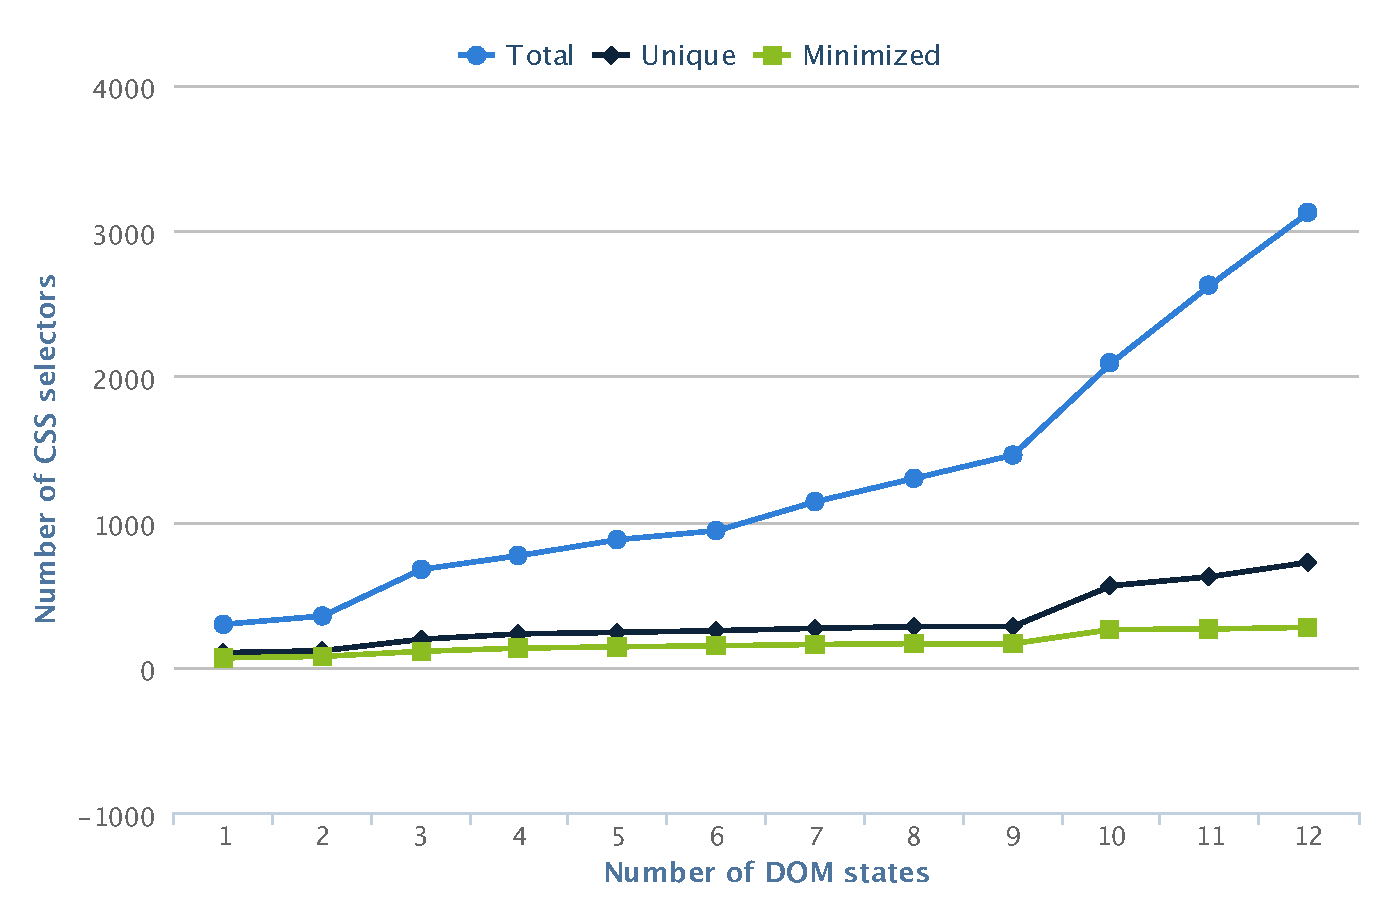
\includegraphics[width=85mm]{images/facebook.pdf}
		\caption{CSS Selectors for user dependent content (Facebook)}
		\label{Fig:Facebook}
	\end{figure}
	\begin{figure}
		\centering
		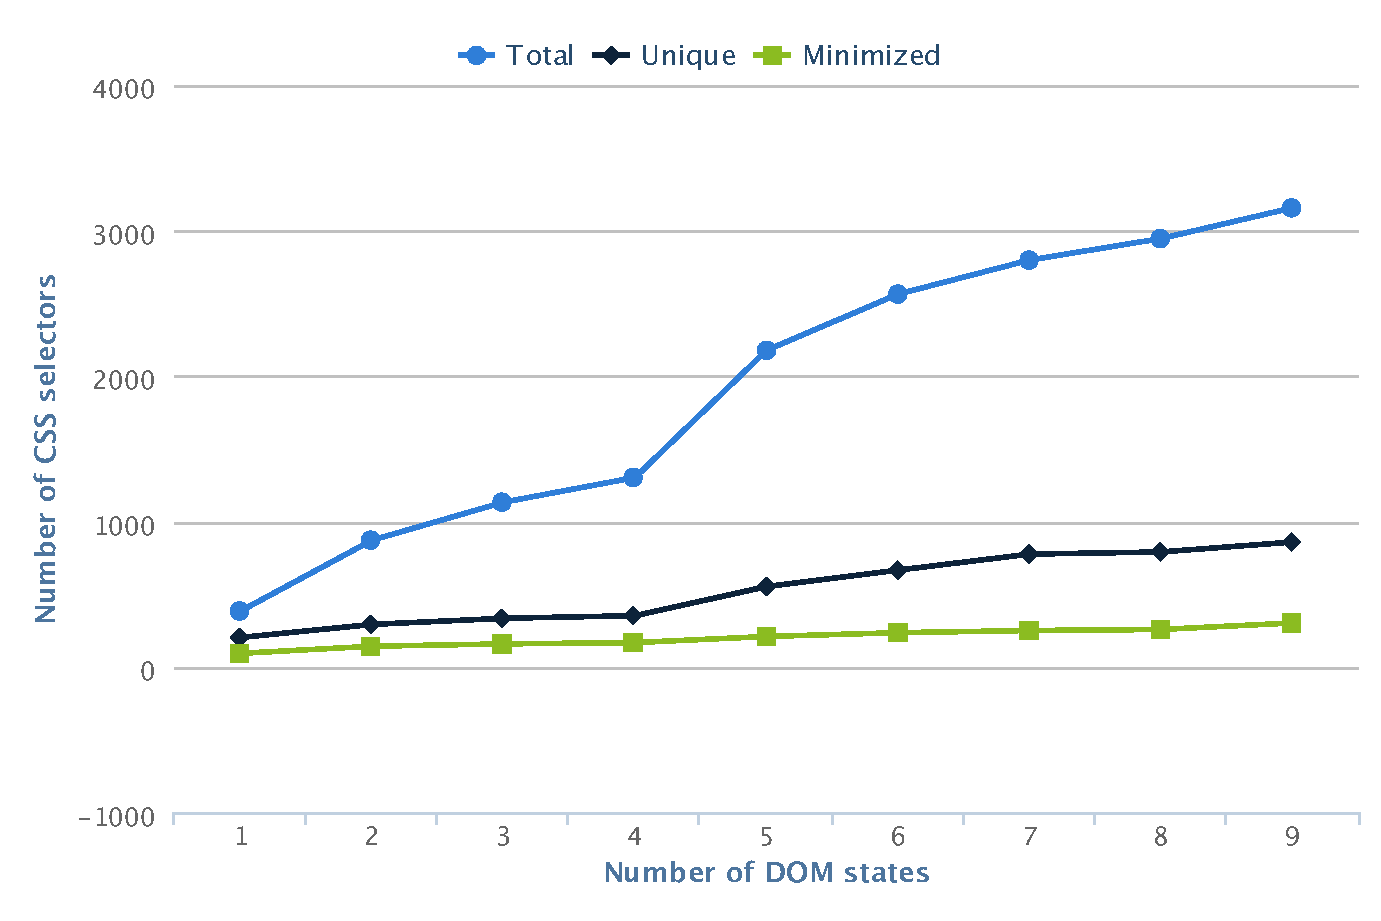
\includegraphics[width=85mm]{images/wikipedia.pdf}
		\caption{CSS Selectors for user generated content (Wikipedia)}
		\label{Fig:Wikipedia}
	\end{figure}
	\begin{figure}
		\centering
		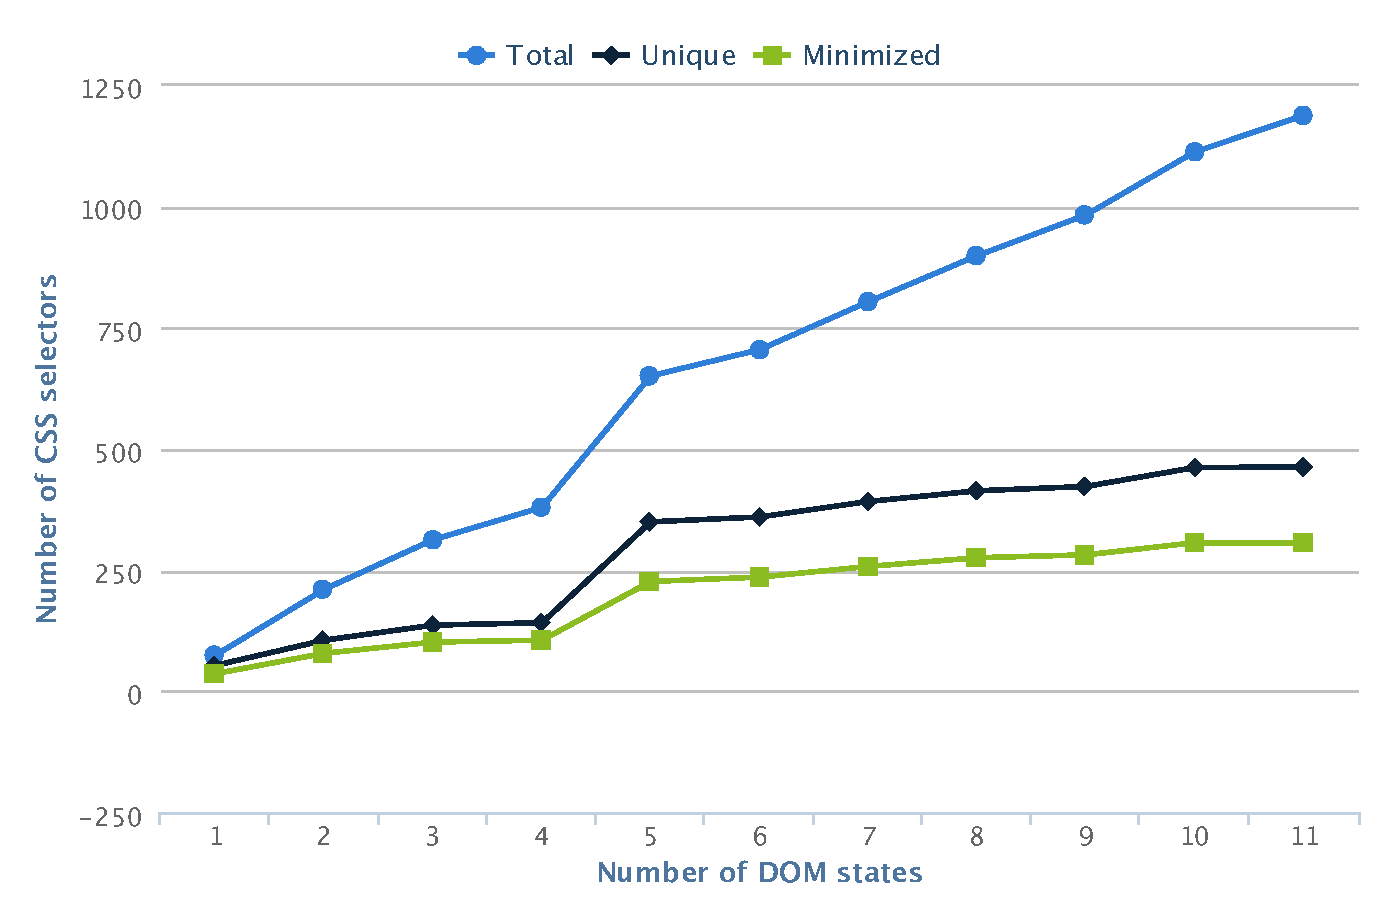
\includegraphics[width=85mm]{images/bing.pdf}
		\caption{CSS Selectors for Search Engine (Bing)}
		\label{Fig:Bing}
	\end{figure}
	\begin{figure}
		\centering
		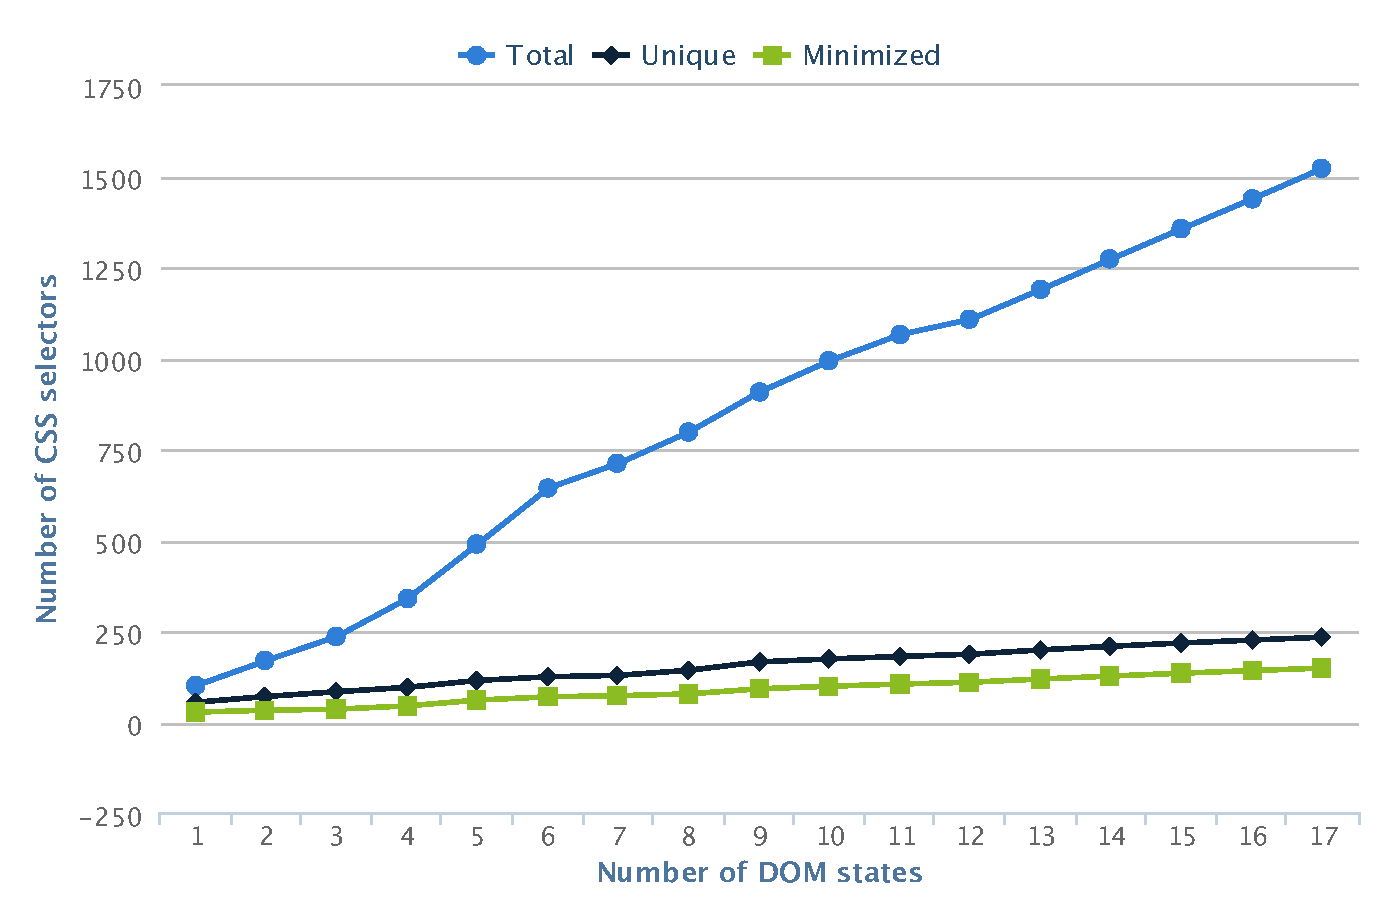
\includegraphics[width=85mm]{images/wordpress.pdf}
		\caption{CSS Selectors for blog (Wordpress)}
		\label{Fig:Wordpress}
	\end{figure}
	\begin{figure}
		\centering
		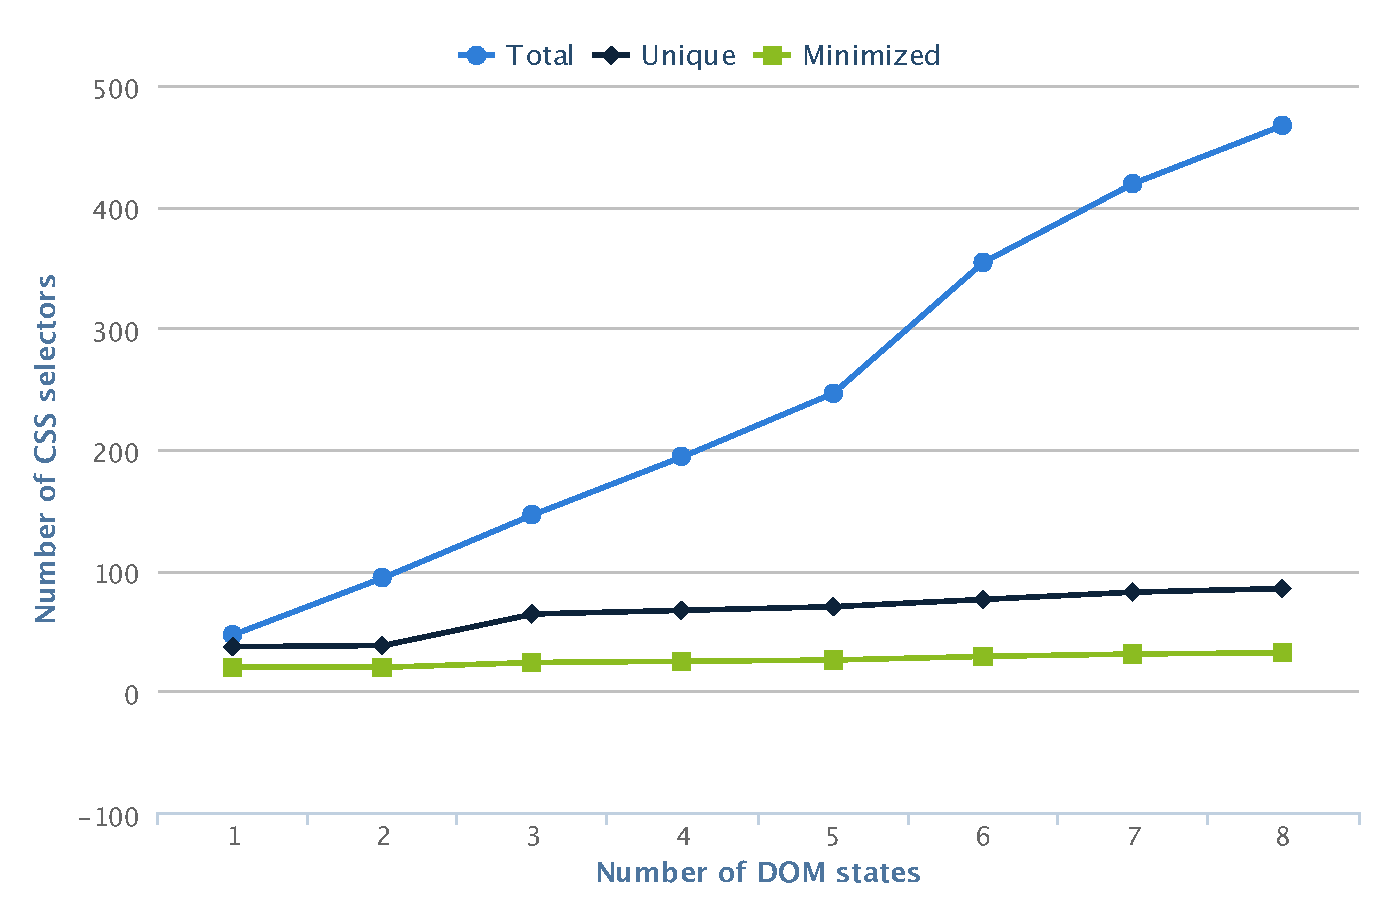
\includegraphics[width=85mm]{images/ajax.pdf}
		\caption{CSS Selectors for AJAX based website (Blog)}
		\label{Fig:AJAX}
	\end{figure}
	
	\subsection{Convergence rate for \css selectors}
	\label{Sec:Convergence}
	To answer RQ1, we crawled 5 web applications: Facebook\footnote{\url{https://www.facebook.com/}} (User specific content), Wikipedia\footnote{\url{https://www.wikipedia.org/}} (User generated content), Bing\footnote{\url{http://www.bing.com/}} (Search Engine), Wordpress Blog\footnote{\url{http://blogs.ubc.ca/karthik/}} and AJAX based blog\footnote{\url{http://www.ece.ubc.ca/~amesbah/}}. All the applications chosen for analysis were dynamic in nature, \ie the DOM tree generated for these websites is either user or input dependent. We also analyzed two blogs where content of DOM tree is dependent on one single user (blog admin) and similar for other user. 
	
	For each web application, we started crawling their home page. We counted the total number of \css selectors, total number of unique \css selectors and total number of minimized \css selectors. For every successive DOM states we included the list of \css selectors from the previous states, therefore only measuring the new \css selectors encountered at each state. 
	
	\figref{Facebook} - \ref{Fig:AJAX} represent the results of analysis at the  end of each DOM state for different websites. As seen from the results, all of the above mentioned websites exhibit patterns in their \css selectors and these patterns tend to converge quickly. The patterns once detected can be used to predict the structure of DOM states that were not encountered during the crawling phase. Therefore, the code-completion system can detect patterns and provide suggestions even for the unseen but similar DOM states.
	
	\finding{DOM states for a particular website exhibit patters in their \css selectors and these patterns tend to converge with increasing number of DOM states. \label{Finding:Convergence}}
	
	
	\begin{figure}
		\centering
		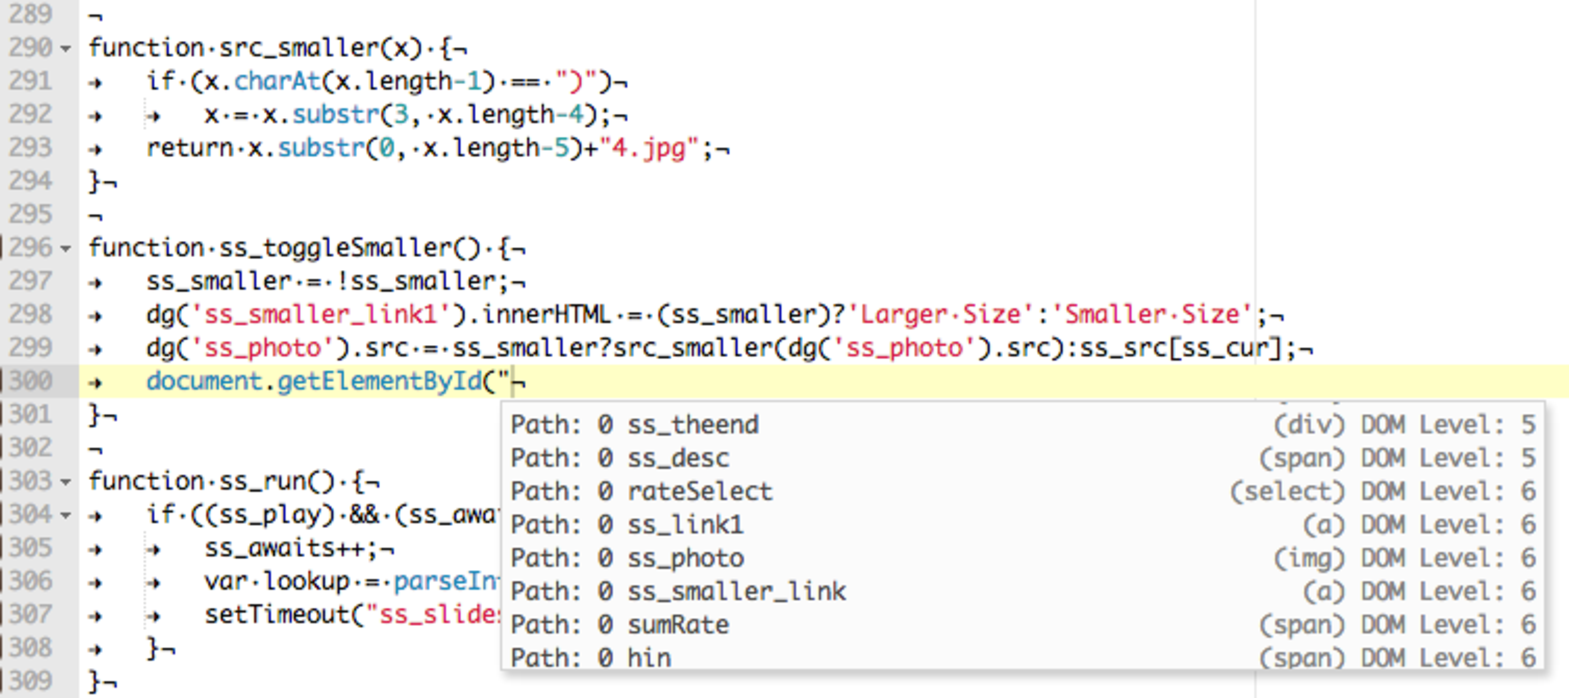
\includegraphics[width=85mm]{images/accuracy.pdf}
		\caption{Code completion suggestions generated using \dompletion}
		\label{Fig:Accuracy}
	\end{figure}
	
	\begin{table}
	{
		\scriptsize
		\begin{tabular}{ p{3.8cm} | p{3.8cm}}
  			\hline                        
  			\textbf{Output} & \textbf{No. of use cases} \\ \hline \hline
  			Valid Suggestions &  40 \\ \hline
			Invalid Suggestions & 7 \\ \hline
			Error & 6 \\ \hline
			Total & 53 \\ 
			\hline  
		\end{tabular}
	}
	\caption {\dompletion evaluation}
	\label{Table:Accuracy}		
	\end{table}
	
	
	
	
	\subsection{Accuracy of \dompletion}
	\label{Sec:Accuracy}
	To answer RQ2, we performed our analysis using an existing php-\javascript based web application Phormer\footnote{\url{http://p.horm.org/er/}}. The choice of web application was based on the following factors:
	\begin{itemize}
		\item \textbf{No use of \javascript libraries:} As our tool \dompletion is in the beginning phase of development, we do not support \javascript libraries. Therefore we prefer to use a web application that does not use libraries. Also we first need to evaluate out tool using native \javascript functions followed by the extension to support \javascript libraries. We discuss about this in detail in \secref{Discussion}.
		
		\item \textbf{Single \javascript file:} All the \javascript code used within this web application was available within a single \javascript file. Therefore making the analysis easier.
		
		\item \textbf{Representative code sample:} The \javascript code used within this application is a representative for a general \javascript code that actively interacts with the DOM. The \javascript file contains 315 lines of code which is good enough for the analysis.
		
	\end{itemize}
	
	In total, there were 53 calls to the \texttt{getElementById} function within the \javascript code. We tried to generate code-completion suggestions for all the calls.    \figref{Accuracy} represents the valid output where the list of suggestions contain the ID that was used within the code. We used the code-completion tool to generate suggestions at Line 300, and see if the element ID used at Line 299 is available in the suggestions. 
	
	\tabref{Accuracy} represents the results of our analysis. As seen from the results, \dompletion can provide code completion suggestions with an accuracy of about 75\%. \dompletion was not able to generate suggestions for some of the \texttt{getElementById} function calls. This was due to the fact that some of the DOM states were not at all explored during the DOM analysis phase. However, a brief information about the web application can improve this accuracy. We also encountered some error cases while analyzing the code. One major reason was improper handling of function parameters. We plan to improve upon these in the next version of our tool.
	
	\finding{\dompletion can provide code-completion suggestions with an accuracy of about 75\% and this accuracy can be improved using application specific information. \label{Finding:Accuracy}}
	
	\subsection{No. of Suggestions}
	\label{Sec:Suggestions}
	To answer RQ3, we used the same \javascript code as in \secref{Accuracy}
